\documentclass{article}
\usepackage[utf8]{inputenc}
\usepackage{uncial}
\usepackage{blindtext}
\usepackage{biblatex}
\usepackage{graphicx}
\addbibresource{Quellen.bib}
%\usepackage{geometry}
%\geometry{
%outer=10mm,
%inner=15mm,
%top=20mm,
%bottom=40mm}

\title{Einführung in die Medieninformatik Woche 8}
\author{Leon Schreiber}
\date{Dezember 2021}

\begin{document}

\maketitle

\newpage

\section{Schrift}
Es gibt verschiedene Schriftgrößen. \\\\
% Die Befehle dafür sind wie Schalter. Wenn man sie "angeschaltet" hat, dann bleiben sie aktiv, bis man etwas Anderes einstellt.
\tiny tiny \\
... \\
\small small \\
... \\
\large large \\
... \\
\huge huge \\
Ab jetzt ist alles huge! Man muss es erst wieder ausstellen.
\\
\normalsize Wieder normal :)
\\\\
\textbf{fett} \textit{kursiv} \textsc{Small Caps}
\\\\
\textit{\textbf{Fett UND kursiv! Wow}}
\\\\
\unclfamily Mittelalter Bogenschütze Lalala
\\\\
\normalfont Jetzt ist wieder normal

\newpage

\section{Dokumentenstruktur}
Hier lernen wir über Struktur
\subsection{Erster Teil}
Im ersten Teil geht es um den ersten Teil des Ganzen
\subsubsection{Blubb}
Fische machen blubb
\subsubsection{Muh}
Kühe machen muh
\subsection{Zweiter Teil}
Der zweite Teil ist etwas besser als der erste Teil.
\paragraph{Wieso?}
Weil er paragraphs enthält
\paragraph{Was ist das?}
Diese coole Einrückung mit dem fetten Text davor

\newpage

\section{Textstruktur}
\begin{center}
Zentrierter Text ist sehr schön
\end{center}
Danach sieht alles wieder ganz normal aus \marginpar{Dazu noch kleine Randnotiz}
\begin{flushright}
Und rechtsbündig kann man dann auch schreiben, cool
\end{flushright}
\\\\
So sieht es aus, wenn man Zitate einfügt:\\
\begin{quote}
    Wenn ich mich zwischen \LaTeX und Atmen entscheiden müsste, würde ich \LaTeX nehmen! \\ \textit{H. Müller} \footnote{Zitat leicht abgeändert und das hier ist eine Fußnote}
\end{quote}
\vspace{2cm}
Hierüber ist ein vertikaler Abstand. Jetzt zählen wir Gemüse auf:
\begin{itemize}
    \item Zwiebeln
    \begin{itemize}
        \item Gelbe
        \item Rote
    \end{itemize}
    \item Knoblauch \cite{mustermann.1996}
    \item Kartoffeln\\
\end{itemize}
Hinter \textit{Knoblauch} sehen wir eine Zitierung. Das ist Wissenschaft.

\newpage

\section{Tabellen}
Mit \LaTeX können wir auch schöne Tabellen machen\\\\
\begin{table}[h!]
    \centering
    \begin{tabular}{l|c|c}
       Name & Kann & Wie gut? \\\hline\hline
        Notepad & Nicht viel & meh \\
        MS Word & Bissle was & schon gut \\
        \LaTeX & Alles & Extrem sexy
    \end{tabular}
    \caption{So schön können Tabellen sein!}
    \label{tabelle1}
\end{table}
\\\\
Später können wir uns sogar wieder auf unsere Tabellen beziehen: \\\\

Tabelle \ref{tabelle1} auf Seite \pageref{tabelle1} zeigt: \LaTeX ist cool.

\newpage

\section{Grafiken}

\begin{figure}[h!]
     \centering
     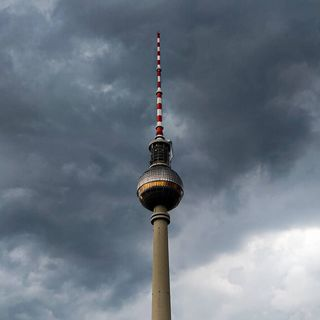
\includegraphics[width=0.2\textwidth]{alex.jpg}
     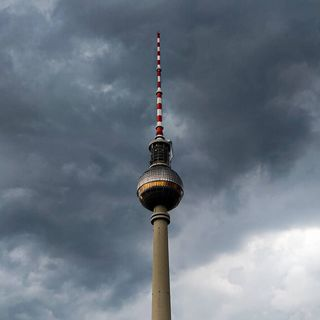
\includegraphics[scale=0.1]{alex.jpg}{}
     \caption{Das ist ein Testbild}
     \label{fig:testbild}
 \end{figure}

\newpage

\printbibliography

\end{document}
